\section{Introduction}

Bubbles within liquids are incredibly common, occurring in both a wide spectrum of natural and industrial processes \cite{Volcano,bird2010daughter,deike2022mass,dollet2019bubble,feng2014nanoemulsions,oratis2020new,veron2015ocean,WINE}. These occurrences can range from water and carbon-dioxide bubbles in magma providing driving forces for an eruption \cite{Volcano} to carbon-dioxide bubbles in champagne enhancing the evaporation of volatile organic compounds dispersed in the liquid phase. When a bubble rises to the surface of a liquid, it may burst, scattering many droplets. These droplets are an important process of transport exchange across the liquid gas interface\cite{notdoneyet}, they are considered the main source of sea spray aerosols and impact air pollution[] as well as the transmission of infectious diseases[]. Bubbles formed due to the breaking of waves contribute to the transfer of heat, mass and other contaminants between the oceans and the atmosphere. The efficiency of this transfer is governed by the initial size and speed of the ejected drops.

There are two Phenomena that occur when a bubble bursts that produce aerosols, the first being when the thin film separating the bubble from the atmosphere is ruptured. The atomisation of the film can produce several hundred droplets of around a micrometer in diameter. Due to the length scales of the rupture being order O($100$nm), we are unable to describe this problem with continuum mechanics. In fact, van der Waals forces or electrostatic repulsion must be considered, both of which are long-range intermolecular forces.

After the film rupture, the remaining cavity collapses causing a jet to form. This jet eventually breaches into one or more droplets. The key difference between these droplets and the droplets formed when the film ruptures is that they are much larger, order O($100 \mu$m) for a typical bubble with a diameter of a millimeter. They are also ejected vertically with a typical ejection velecity of order O($1$ms$^{-1}$).
\begin{figure}[hb]
    \centering
    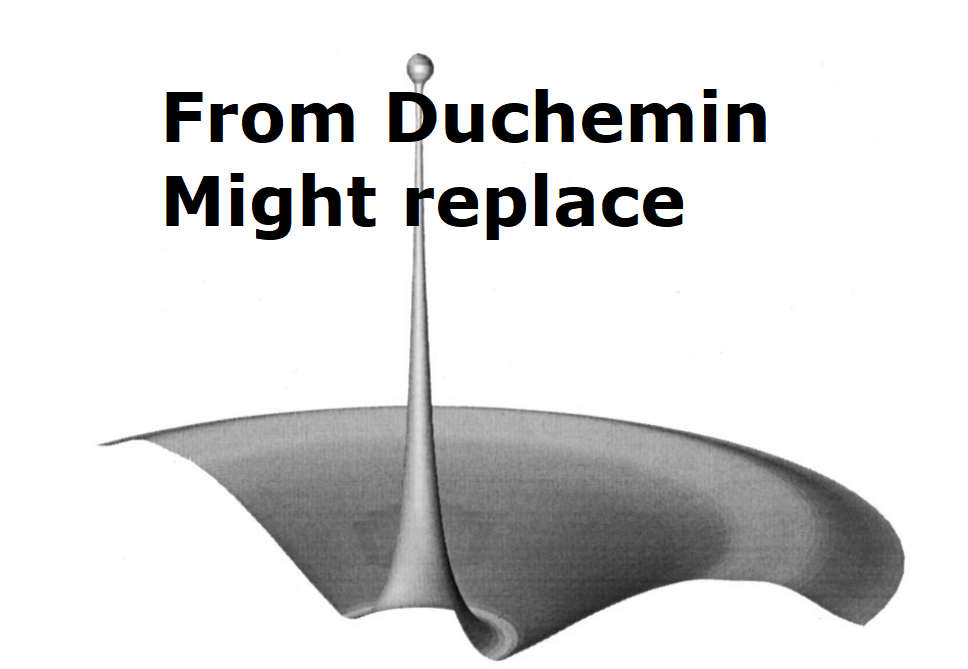
\includegraphics[width=0.55\linewidth]{WriteUp/images/Untitled.png}
    \caption{An image of jet formation due to a burst bubble}
    \label{fig:1}
\end{figure}

Literature review goes here:


just some notes:

\begin{align*}
We = \frac{\rho v^2 L}{\sigma}\\
La = \frac{\sigma \rho L}{\mu^2} \\
Re = \sqrt{LaWe}\\
Bo = \frac{\Delta \rho g L^2}{\sigma}\\
Oh = (La)^{-0.5})\\
\end{align*}
